\documentclass{article}
\usepackage[margin=1in]{geometry}
\usepackage{amsmath}
\usepackage{amssymb}
\usepackage{graphicx}
\usepackage{mathtools}
\usepackage{tikz}
\graphicspath{images/}

\newcommand{\R}{\mathbb{R}}
\newcommand{\abs}[1]{\left\vert #1 \right\vert}

\begin{document}

\title{Piecewise Polynomials with Bounded Derivatives}
\author{Aresh Pourkavoos}
\maketitle

I originally encountered this problem on my high school robotics team.
We wanted to program a routine for our robot
to move from one point to another in a straight line in the minimum time $T$.
For simplicity, assume the robot
is moving in one dimension by a distance $d_0 > 0$.
The robot has a top speed $d_1 > 0$,
so the most straightforward routine is
to calculate the time it takes to travel the desired distance at top speed
(i.e. $T=\frac{d_1}{d_0}$)
and to run the motors for that length of time.
The velocity and position graphs for this routine are below.
\begin{center}
  \begin{tikzpicture}[scale=0.5]
    \begin{scope}[shift={(0,0)}]
      \draw[->] (-1.5, 0) -- (4.5, 0) node[right] {$t$};
      \draw[->] (0, -0.5) -- (0, 6.5) node[above] {$v$};
      \draw (0.25, 2) -- (-0.25, 2) node[left] {$d_1$};
      \draw (3, 0.25) -- (3, -0.25) node[below] {$T$};
      \draw[very thick, color=red] plot coordinates {(-1, 0) (0, 0) (0, 2) (3, 2) (3, 0) (4, 0)};
    \end{scope}
    \begin{scope}[shift={(8,0)}]
      \draw[->] (-1.5, 0) -- (4.5, 0) node[right] {$t$};
      \draw[->] (0, -0.5) -- (0, 6.5) node[above] {$x$};
      \draw (0.25, 6) -- (-0.25, 6) node[left] {$d_0$};
      \draw (3, 0.25) -- (3, -0.25) node[below] {$T$};
      \draw[very thick, color=red] plot coordinates {(-1, 0) (0, 0) (3, 6) (4, 6)};
    \end{scope}
  \end{tikzpicture}
\end{center}
However, this solution was unsatisfactory
because of the sudden acceleration from rest to top speed,
which would cause the wheels to slip
and the distance traveled to be inconsistent.
So we placed a limit $d_2 > 0$ on the acceleration,
had the robot accelerate at that rate to top speed,
maintain that speed for as long as possible,
then slow down to rest as it approached the destination.
The new graphs of acceleration, velocity, and position were:
\begin{center}
  \begin{tikzpicture}[scale=0.5]
    \begin{scope}[shift={(0,0)}]
      \draw[->] (-1.5, 0) -- (5.5, 0) node[right] {$t$};
      \draw[->] (0, -2.5) -- (0, 6.5) node[above] {$a$};
      \draw (0.25, 2) -- (-0.25, 2) node[left] {$d_2$};
      \draw (4, -0.25) -- (4, 0.25) node[above] {$T$};
      \draw[very thick, color=red] plot coordinates {(-1, 0) (0, 0) (0, 2) (1, 2) (1, 0) (3, 0) (3, -2) (4, -2) (4, 0) (5, 0)};
    \end{scope}
    \begin{scope}[shift={(9,0)}]
      \draw[->] (-1.5, 0) -- (5.5, 0) node[right] {$t$};
      \draw[->] (0, -2.5) -- (0, 6.5) node[above] {$v$};
      \draw (0.25, 2) -- (-0.25, 2) node[left] {$d_1$};
      \draw (4, 0.25) -- (4, -0.25) node[below] {$T$};
      \draw[very thick, color=red] plot coordinates {(-1, 0) (0, 0) (1, 2) (3, 2) (4, 0) (5, 0)};
    \end{scope}
    \begin{scope}[shift={(18,0)}]
      \draw[->] (-1.5, 0) -- (5.5, 0) node[right] {$t$};
      \draw[->] (0, -2.5) -- (0, 6.5) node[above] {$x$};
      \draw (0.25, 6) -- (-0.25, 6) node[left] {$d_0$};
      \draw (4, 0.25) -- (4, -0.25) node[below] {$T$};
      \draw[very thick, color=red] plot coordinates {(-1, 0) (0, 0)};
      \draw[very thick, color=red, domain=0:1] plot (\x, \x*\x);
      \draw[very thick, color=red] plot coordinates {(1, 1) (3, 5)};
      \draw[very thick, color=red, domain=3:4] plot (\x, -10+8*\x-\x*\x);
      \draw[very thick, color=red] plot coordinates {(4, 6) (5, 6)};
    \end{scope}
  \end{tikzpicture}
\end{center}
However, over short enough distances,
the robot would not have enough time to reach full speed,
so it would need to begin decelerating before then:
\begin{center}
  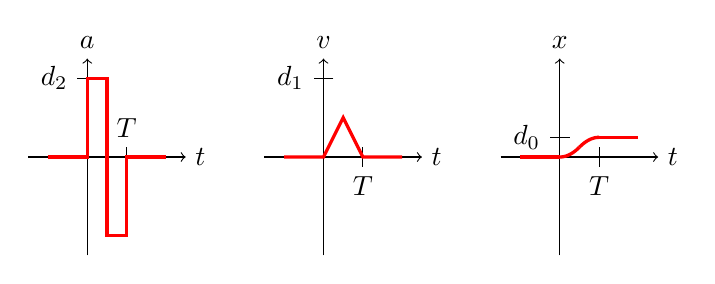
\begin{tikzpicture}[scale=0.5]
    \begin{scope}[shift={(0,0)}]
      \draw[->] (-1.5, 0) -- (2.5, 0) node[right] {$t$};
      \draw[->] (0, -2.5) -- (0, 2.5) node[above] {$a$};
      \draw (0.25, 2) -- (-0.25, 2) node[left] {$d_2$};
      \draw (1, -0.25) -- (1, 0.25) node[above] {$T$};
      \draw[very thick, color=red] plot coordinates {(-1, 0) (0, 0) (0, 2) (0.5, 2) (0.5, -2) (1, -2) (1, 0) (2, 0)};
    \end{scope}
    \begin{scope}[shift={(6,0)}]
      \draw[->] (-1.5, 0) -- (2.5, 0) node[right] {$t$};
      \draw[->] (0, -2.5) -- (0, 2.5) node[above] {$v$};
      \draw (0.25, 2) -- (-0.25, 2) node[left] {$d_1$};
      \draw (1, 0.25) -- (1, -0.25) node[below] {$T$};
      \draw[very thick, color=red] plot coordinates {(-1, 0) (0, 0) (0.5, 1) (1, 0) (2, 0)};
    \end{scope}
    \begin{scope}[shift={(12,0)}]
      \draw[->] (-1.5, 0) -- (2.5, 0) node[right] {$t$};
      \draw[->] (0, -2.5) -- (0, 2.5) node[above] {$x$};
      \draw (0.25, 0.5) -- (-0.25, 0.5) node[left] {$d_0$};
      \draw (1, 0.25) -- (1, -0.25) node[below] {$T$};
      \draw[very thick, color=red] plot coordinates {(-1, 0) (0, 0)};
      \draw[very thick, color=red, domain=0:0.5] plot (\x, \x*\x);
      \draw[very thick, color=red, domain=0.5:1] plot (\x, -0.5+2*\x-\x*\x);
      \draw[very thick, color=red] plot coordinates {(1, 0.5) (2, 0.5)};
    \end{scope}
  \end{tikzpicture}
\end{center}

$T$ still represents the total time to excecute the maneuver,
but its formula has changed.
The time to accelerate to top speed is given by $\frac{d_1}{d_2}$,
and the distance the robot travels in that time is
$\frac{d_2}{2}\left(\frac{d_1}{d_2}\right)^2=\frac{d_1^2}{2d_2}$.
If the total distance traveled is at least twice that,
i.e. if $d_0 \geq \frac{d_1^2}{d_2}$,
then the robot can reach top speed on the way.
Thus it spends $\frac{2d_1}{d_2}$ time accelerating and decelerating (altogether),
and the distance it covers at top speed is $d_0-\frac{d_1^2}{d_2}$, which takes
$\frac{1}{d_1}\left(d_0-\frac{d_1^2}{d_2}\right)=\frac{d_0}{d_1}-\frac{d_1}{d_2}$ time.
Then $T=\frac{2d_1}{d_2}+\frac{d_0}{d_1}-\frac{d_1}{d_2}=\frac{d_0}{d_1}+\frac{d_1}{d_2}$.
On the other hand, if $d_0 < \frac{d_1^2}{d_2}$,
the robot can only accelerate until it is halfway to the destination,
which also takes half of the total time
(as the other half is spent slowing back down).
Thus $\frac{d_0}{2}=\frac{d_2}{2}\left(\frac{T}{2}\right)^2$,
so $T=2\sqrt{\frac{d_0}{d_2}}$.

This solution worked well enough for our robot,
but some applications also place a limit $d_3 > 0$ on jerk,
which is the third derivative of position with respect to time,
i.e. the rate of change of acceleration.
For example, people in elevators feel acceleration as weight,
so if the elevator jumps from rest to some nonzero acceleration,
the passengers will feel a sudden weight change.
As a result, the path of an elevator
may have up to 7 polynomial pieces.
Example jerk, acceleration, velocity, and position curves
are shown below.

\begin{center}
  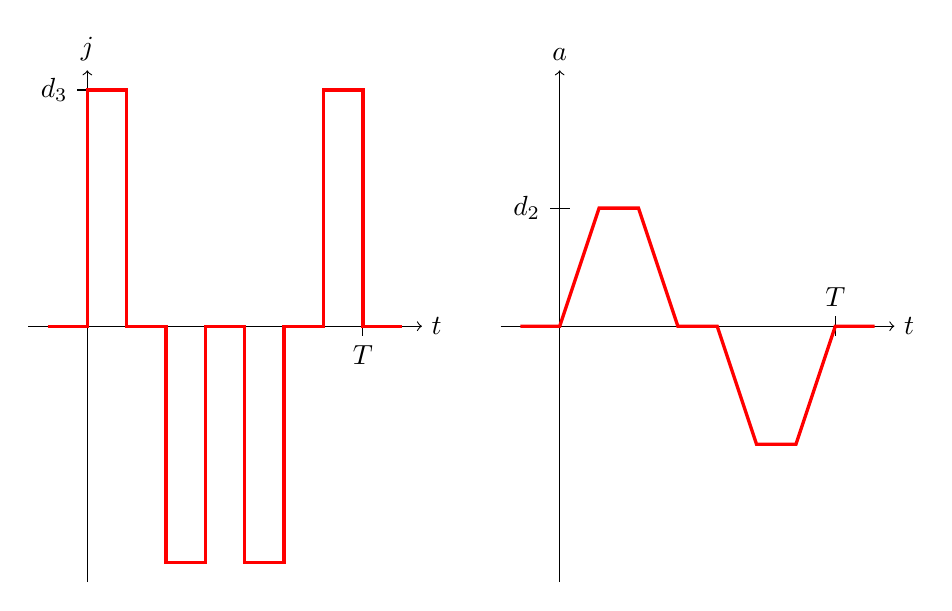
\begin{tikzpicture}[xscale=0.5,yscale=0.0625]
    \begin{scope}[shift={(0,0)}]
      \draw[->] (-1.5, 0) -- (8.5, 0) node[right] {$t$};
      \draw[->] (0, -52) -- (0, 52) node[above] {$j$};
      \draw (0.25, 48) -- (-0.25, 48) node[left] {$d_3$};
      \draw (7, 2) -- (7, -2) node[below] {$T$};
      \draw[very thick, color=red] plot coordinates {(-1, 0) (0, 0) (0, 48) (1, 48) (1, 0) (2, 0) (2, -48) (3, -48) (3, 0) (4, 0) (4, -48) (5, -48) (5, 0) (6, 0) (6, 48) (7, 48) (7, 0) (8, 0)};
    \end{scope}
    \begin{scope}[shift={(12,0)}]
      \draw[->] (-1.5, 0) -- (8.5, 0) node[right] {$t$};
      \draw[->] (0, -52) -- (0, 52) node[above] {$a$};
      \draw (0.25, 24) -- (-0.25, 24) node[left] {$d_2$};
      \draw (7, -2) -- (7, 2) node[above] {$T$};
      \draw[very thick, color=red] plot coordinates {(-1, 0) (0, 0) (1, 24) (2, 24) (3, 0) (4, 0) (5, -24) (6, -24) (7, 0) (8, 0)};
    \end{scope}
  \end{tikzpicture} \\
  \vspace{5mm}
  \begin{tikzpicture}[xscale=0.5,yscale=0.0625]
    \begin{scope}[shift={(0,0)}]
      \draw[->] (-1.5, 0) -- (8.5, 0) node[right] {$t$};
      \draw[->] (0, -4) -- (0, 52) node[above] {$v$};
      \draw (0.25, 24) -- (-0.25, 24) node[left] {$d_1$};
      \draw (7, 2) -- (7, -2) node[below] {$T$};
      \draw[very thick, color=red] plot coordinates {(-1, 0) (0, 0)};
      \draw[very thick, color=red, domain=0:1] plot (\x, 6*\x*\x);
      \draw[very thick, color=red] plot coordinates {(1, 6) (2, 18)};
      \draw[very thick, color=red, domain=2:3] plot (\x, -6*\x*\x+36*\x-30);
      \draw[very thick, color=red] plot coordinates {(3, 24) (4, 24)};
      \draw[very thick, color=red, domain=4:5] plot (\x, -6*\x*\x+48*\x-72);
      \draw[very thick, color=red] plot coordinates {(5, 18) (6, 6)};
      \draw[very thick, color=red, domain=6:7] plot (\x, 6*\x*\x-84*\x+294);
      \draw[very thick, color=red] plot coordinates {(7, 0) (8, 0)};
    \end{scope}
    \begin{scope}[shift={(12,0)}]
      \draw[->] (-1.5, 0) -- (8.5, 0) node[right] {$t$};
      \draw[->] (0, -4) -- (0, 52) node[above] {$x$};
      \draw (0.25, 48) -- (-0.25, 48) node[left] {$d_0$};
      \draw (7, 2) -- (7, -2) node[below] {$T$};
      \draw[very thick, color=red] plot coordinates {(-1, 0) (0, 0)};
      \draw[very thick, color=red, domain=0:1] plot (\x, \x*\x*\x);
      \draw[very thick, color=red, domain=1:2] plot (\x, 3*\x*\x-3*\x+1);
      \draw[very thick, color=red, domain=2:3] plot (\x, -\x*\x*\x+9*\x*\x-15*\x+9);
      \draw[very thick, color=red] plot coordinates {(3, 18) (4, 30)};
      \draw[very thick, color=red, domain=4:5] plot (\x, -\x*\x*\x+12*\x*\x-36*\x+46);
      \draw[very thick, color=red, domain=5:6] plot (\x, -3*\x*\x+39*\x-79);
      \draw[very thick, color=red, domain=6:7] plot (\x, \x*\x*\x-21*\x*\x+147*\x-295);
      \draw[very thick, color=red] plot coordinates {(7, 48) (8, 48)};
    \end{scope}
  \end{tikzpicture}
\end{center}

%% At this point, the general version of the problem 

%% Given an integer $n \geq 1$ and positive real numbers $d_0, d_1, \ldots, d_n$,
%% find the function $x : \R \rightarrow \R$ where

%% \begin{itemize}
%% \item
%%   $x(t)=0$ for all $t \leq 0$;
%% \item
%%   $x(t)=d_0$ for all $t \geq T$, where $T \in \R$;
%% \item
%%   $\abs{x}$ 
%% \end{itemize}

%% which minimizes the value of $T$.

%% In other words, if the first $n$ derivatives of $x$
%% are absolutely bounded by $d_1, \ldots, d_n$,

% Note on Lipschitz

\end{document}
